\documentclass{article}

\usepackage[T1]{fontenc}
\usepackage[utf8]{inputenc}
\usepackage[brazilian]{babel}
\usepackage{graphicx}
\usepackage[export]{adjustbox}[2011/08/13]
\usepackage{float}
\usepackage[pdftex]{hyperref}
\usepackage{epstopdf}
\usepackage{etoolbox}
\usepackage{amsmath}
\usepackage{amsfonts}
\usepackage{amssymb}
\usepackage{caption}
\usepackage{subcaption}
\usepackage{setspace}
\usepackage{tikz}
\usepackage{listings}
\usepackage{xcolor} 

\bibliographystyle{eric}
\patchcmd{\thebibliography}{\section*}{\section}{}{}


\newcommand{\R}{\ensuremath{\mathbb{R}}}
\newcommand{\Prob}{\ensuremath{\mathbb{P}}}
\newcommand{\K}{\ensuremath{\mathbb{K}}}
\newcommand{\U}{\ensuremath{\mathbb{U}}}
\newcommand{\N}{\ensuremath{\mathbb{N}}}
\newcommand{\Lg}{\ensuremath{\mathbb{L}}}
\newcommand{\T}{\ensuremath{\rm Tr}}
\newcommand{\sg}{{\sigma(x_k)}}

\newcommand{\G}{\ensuremath{\mathcal{G}}}
\newcommand{\F}{\ensuremath{\mathcal{F}}}
\newcommand{\C}{\ensuremath{\mathcal{C}}}
\newcommand{\E}{\ensuremath{\mathcal{E}}}
\newcommand{\Hn}{\ensuremath{\mathcal{H}}}
\newcommand{\Hoo}{\ensuremath{\mathcal{H}_\infty}}
\newcommand{\Hop}{\ensuremath{\mathcal{H}_{op}}}
% --------------------------------------------------
\newtheorem{theo}{Teorema}
\newtheorem{exa}{Exemplo}
\newtheorem{lemm}{Lema}
\newtheorem{coro}{Corolário}
\newtheorem{defn}{Definição}[section]

\begin{document}

\begin{titlepage}
\begin{center}

\newcommand{\HRule}{\rule{\linewidth}{0.5mm}}
% Upper part of the page. The '~' is needed because \\
% only works if a paragraph has started.

\includegraphics[width=0.15\textwidth]{logoUnicamp}~\\[1cm]

\textsc{\LARGE Universidade Estadual de Campinas}\\[1.5cm]

\textsc{\Large Faculdade de Engenharia Mecânica}\\[0.5cm]

% Title
\HRule \\[0.4cm]
{ \huge \bfseries ES664 - Laboratório de Eletrônica para Automação Industrial\\ \vspace{1cm} Relatório - Experimento 4\\
\Large{Acionamento de motor DC} \\[0.4cm] }

\HRule \\[1.5cm]

% Author and supervisor
\begin{minipage}{0.6\textwidth}
\begin{flushleft} \large
\emph{Nome:}\\
Daniel Dello Russo Oliveira\\Marcelli Tiemi Kian
\end{flushleft}
\end{minipage}
\begin{minipage}{0.2\textwidth}
\begin{flushright} \large
\emph{RA}\\ 101918\\117892
\end{flushright}
\end{minipage}

\vfill

% Bottom of the page
{\large \today}

\end{center}
\end{titlepage}


\onehalfspacing
\section{Objetivos}
	O experimento tem como objetivo implementar o acionamento de um motor DC através de um retificador controlado e um chopper. Além disso, queremos avaliar o controle de velocidade do motor em malha aberta.
	 
\section{Experimento}
\subsection{Retificador Monofásico Controlado}
Utilizamos um transformador para rebaixar a tensão de $220\ V$ para $24\ V$, fazendo a ligação da tensão de linha (protegida pelos fusíveis) no primário, obtendo como saída $25.54\ V$. No secundário, ligamos o circuito na entrada do conversor. Alimentamos e configuramos o cartão de disparos, permitindo configurar $\alpha$ por meio de um potenciômetro. O esquemático do sistema pode ser visto na figura \ref{fig:retesq}.

\begin{figure}[H]
	\centering
	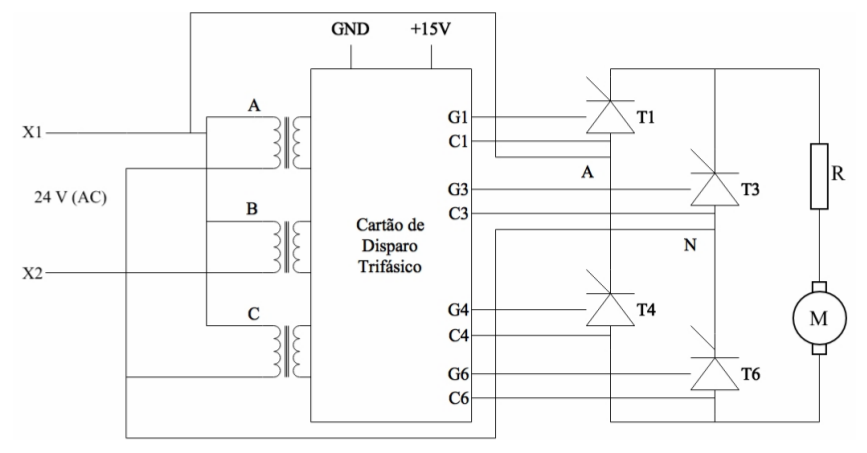
\includegraphics[width=\linewidth]{Dados/Retificador/esq}
	\caption{Retificador monofásico controlado de onda completa utilizado para acionar motor DC. (roteiro)}
	\label{fig:retesq}
\end{figure}

Prosseguimos o experimento com a medição da resistência de armadura do motor:
\begin{equation}
R_a=7.9\ \Omega
\end{equation}
e com a resistência de medição 
\begin{equation}
R_R=3.8\ \Omega
\end{equation}
sendo este último valor diferente do sugerido no roteiro ($0.2\Omega$).

Ligamos o circuito e capturamos a forma de onda da tensão de armadura $v_a$ para $\alpha=90^\circ$, conforme figura \ref{fig:varet}. Variando os valores de $\alpha$, obtivemos os valores da tabela \ref{tab:varet}.

\begin{figure}[H]
	\centering
	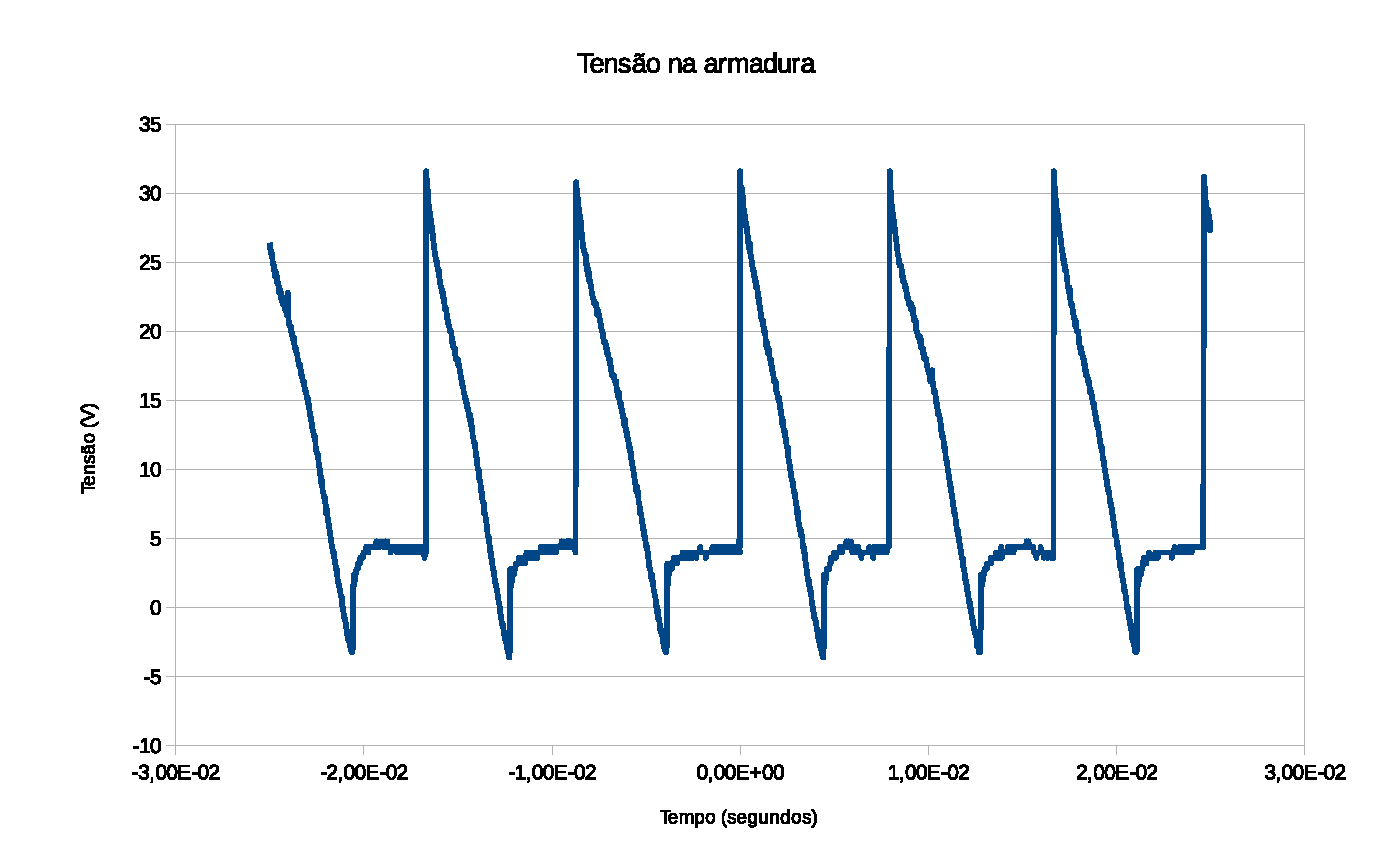
\includegraphics[width=\linewidth]{Dados/Retificador/1}
	\caption{Tensão de armadura do motor DC com retificador controlado para $\alpha=90^\circ$}
	\label{fig:varet}
\end{figure}

\begin{table}[H]
	\centering
	\caption{Tensão de armadura $v_a$ e velocidade angular $\omega_m$ do motor DC para diferentes ângulos de disparo $\alpha$}
	\label{tab:varet}
	\begin{tabular}{|l|l|l|}
		\hline
		$\alpha$ & $v_a$ & $\omega_m$ \\ \hline
		$60^\circ$    & 4.81  & 340        \\ \hline
		$70^\circ$    & 5.9   & 470        \\ \hline
		$80^\circ$    & 7.12  & 650        \\ \hline
		$90^\circ$    & 8.5   & 900        \\ \hline
		$100^\circ$   & 9.8   & 1150       \\ \hline
		$110^\circ$   & 10.6  & 1350       \\ \hline
		$120^\circ$   & 11.6  & 1510       \\ \hline
	\end{tabular}
\end{table}

Medimos também a tensão no resistor de medição $R_R$, para cálculo da corrente de armadura, conforme figura \ref{fig:iaret}.
\begin{figure}[H]
	\centering
	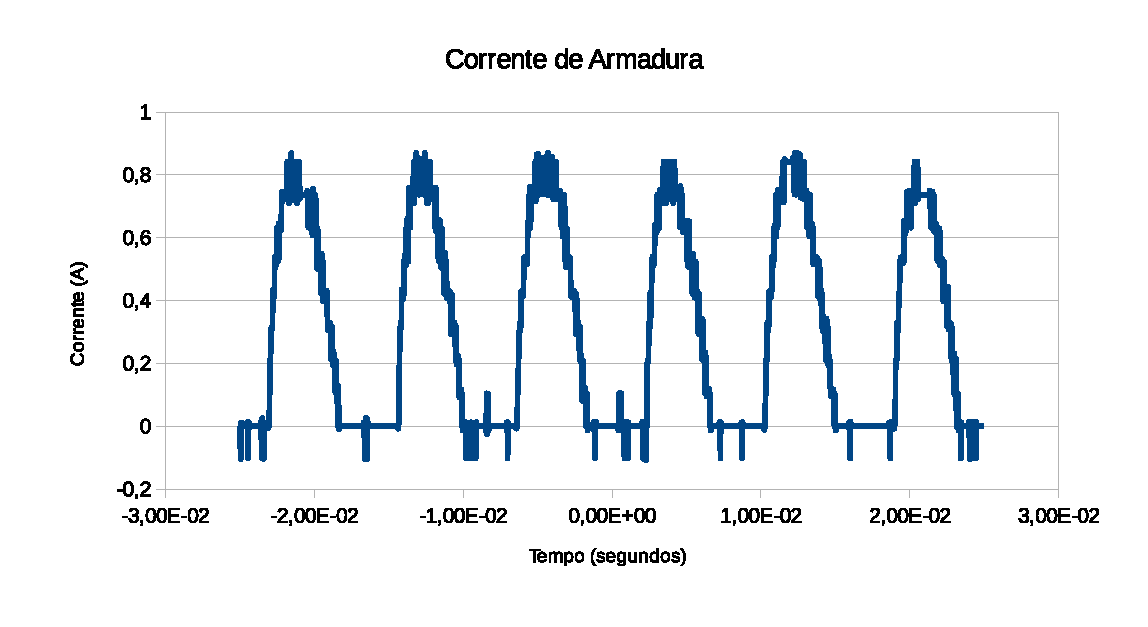
\includegraphics[width=\linewidth]{Dados/Retificador/corrente}
	\caption{Corrente no resistor de medição para $\alpha=90^\circ$}
	\label{fig:iaret}
\end{figure}

Como tivemos problemas na ligação do circuito, descontinuamos o experimento sem fazer a medição da corrente para outros valores de $\alpha$, conforme orientado pelo professor.

\subsection{Conversor Step-Down}
Para o experimento com o conversor step-down, configuramos as tensões da fonte DC e pulsos do gerador de sinal. Ligamos o lado alto do conversor em $12\ V$, e o lado baixo na armadura do motor em série com o resistor de medição. Alimentamos o circuito de acionamento do conversor com $15\ V$ e ligamos o gerador de sinal nos cabos indicados por "BUCK" e "GND".

Utilizamos o mesmo motor do caso anterior, mas outra resistência de medição:

\begin{equation}
R_S=5.3\ \Omega
\end{equation}

Ligamos o circuito e capturamos a forma de onda da tensão de armadura $v_a$ para $D=50\%$, conforme figura \ref{fig:vabuck}. Variando os valores de $D$, obtivemos os valores da tabela \ref{tab:vabuck}.

\begin{figure}[H]
	\centering
	\includegraphics[width=\linewidth]{Dados/Buck/2.bmp}
	\caption{Tensão de armadura do motor DC com chopper em step-down para $D=50\%$}
	\label{fig:vabuck}
\end{figure}

\begin{table}[H]
	\centering
	\caption{Tensão de armadura $v_a$ e velocidade angular $\omega_m$ do motor DC para diferentes duty-cycles $D$}
	\label{tab:vabuck}
	\begin{tabular}{|l|l|l|}
		\hline
		$D$    & $v_a$ & $\omega_m$ \\ \hline
		$20\%$ & -     & -          \\ \hline
		$30\%$ & 2.18  & 102        \\ \hline
		$40\%$ & 3.08  & 234        \\ \hline
		$50\%$ & 4.32  & 390        \\ \hline
		$60\%$ & 5.4   & 574        \\ \hline
	\end{tabular}
\end{table}

Prosseguimos o experimento registrando os valores de tensão na resistência de medição. A forma de onda capturada para a tensão $v_R$ é mostrada na figura \ref{fig:iabuck}, para realizar o cálculo de $i_a$ da tabela \ref{tab:iabuck}, conforme equação a seguir.

\begin{figure}[H]
	\centering
	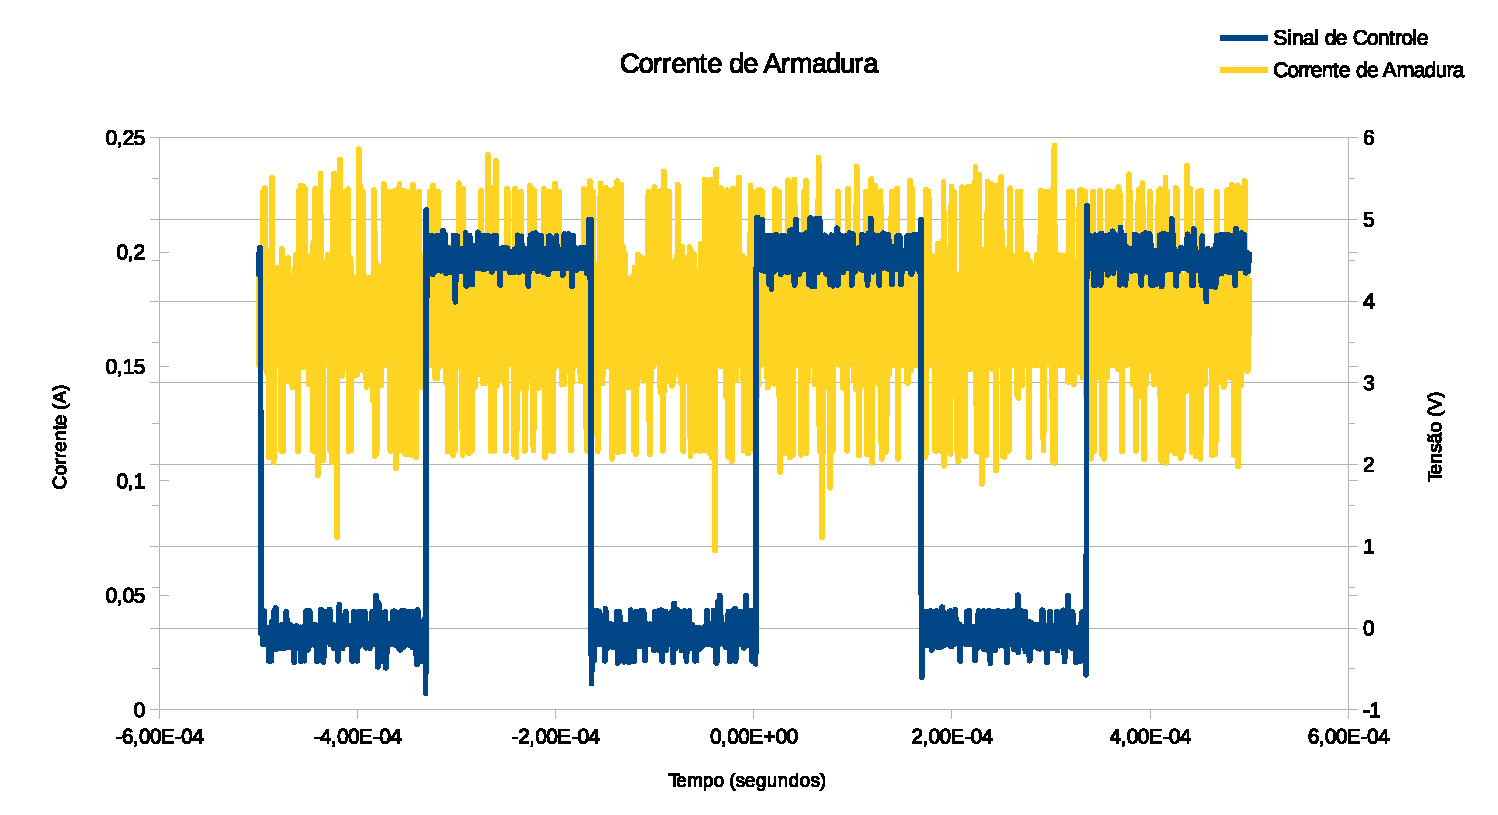
\includegraphics[width=\linewidth]{Dados/Buck/ia.bmp}
	\caption{Tensão no resistor de medição para $D=50\%$}
	\label{fig:iabuck}
\end{figure}

\begin{equation}
i_a=\frac{v_R}{R_S}\ A
\end{equation}

\begin{table}[H]
	\centering
	\caption{Tensão no resistor de medição $v_R$ e corrente de armadura $i_a$ do motor DC para diferentes duty-cycles $D$}
	\label{tab:iabuck}
	\begin{tabular}{|l|l|l|}
		\hline
		$D$    & $v_R$ & $i_a$ \\ \hline
		$20\%$ & -     & -     \\ \hline
		$30\%$ & 0.62  & 0.117 \\ \hline
		$40\%$ & 0.76  & 0.143 \\ \hline
		$50\%$ & 0.9   & 0.170 \\ \hline
		$60\%$ & 1.02  & 0.192 \\ \hline
	\end{tabular}
\end{table}

\end{document}

